\chapter{引用}\label{ch05}

\emph{Libraries cannot provide new inabilities.}

\begin{flushright}
——Mark Miller
\end{flushright}

我们至今为止见过的所有指针类型——简单的\texttt{Box<T>}堆指针、\texttt{String}和\texttt{Vec}内部的指针都拥有值:当所有者被drop时,指针指向的值也会随之消失。Rust还有非拥有指针类型,称为\emph{引用},引用对指向的值的生命周期没有影响。

事实上,正相反,引用绝不应该比它们指向的值活的更长。你必须在你的代码中明确表明,引用的生命寿命比它指向的值更短。为了强调这一点,Rust将创建某个值的引用称为\emph{借用}值:你最终必须把你借走的还给它的所有者。

如果你在读到“你必须在你的代码中明确表明”时感到一丝怀疑,那说明你很优秀。引用自身并没有什么特殊的——本质上,它们只是地址。但保证它们安全的规则是Rust独有的,你以前不可能看到过类似的。尽管这些规则是Rust里最难掌握的部分,但它们能防止的经典的、日常的bug的范围之广令人惊讶,它们对多线程的影响也正在显现。这也是Rust的赌注。

这一章中,我们将讨论Rust中的引用如何工作,展示引用、函数和自定义类型如何包含生命周期信息来保证它们被安全使用,阐释它怎么能在编译期、不引入运行时开销的同时防止常见的bug。

\section{值的引用}

举个例子,假设我们要为文艺复兴时期优秀的艺术家和他们的著名作品建一个表格。Rust的标准库包含一个哈希表类型,所以我们可以像这样定义我们的类型:
\begin{minted}{Rust}
    use std::collections::HashMap;

    type Table = HashMap<String, Vec<String>>;
\end{minted}

换句话说,这是一个把\texttt{String}值映射到\texttt{Vec<String>}值的哈希表,它把艺术家的名字关联到它们的作品的名字。你可以使用\texttt{for}循环来迭代\texttt{HashMap}的条目,因此我们可以写一个函数打印出一个\texttt{Table}:
\begin{minted}{Rust}
    fn show(table: Table) {
        for (artist, works) in table {
            println!("works by {}:", artist);
            for work in works {
                println!("  {}", work);
            }
        }
    }
\end{minted}

构造和打印表格都很直观:
\begin{minted}{Rust}
    fn main() {
        let mut table = Table::new();
        table.insert("Gesualdo".to_string(),
                     vec!["many madrigals".to_string(),
                          "Tenebrae Responsoria".to_string()]);
        table.insert("Caravaggio".to_string(),
                     vec!["The Musicians".to_string(),
                          "The Calling of St. Matthew".to_string()]);
        table.insert("Cellini".to_string(),
                     vec!["Perseus with the head of Medusa".to_string(),
                          "a salt cellar".to_string()]);
        show(table);
    }
\end{minted}

它也能正常工作:
\begin{minted}{text}
    $ cargo run
         Running `/home/jimb/rust/book/fragments/target/debug/fragments`
    works by Gesualdo:
      many madrigals
      Tenebrae Responsoria
    works by Cellini:
      Perseus with the head of Medusa
      a salt cellar
    works by Caravaggio:
      The Musicians
      The Calling of St. Matthew
\end{minted}

但如果你阅读过上一章中有关move的小节,你就会发现\texttt{show}的定义有一些问题。首先,\texttt{HashMap}不是\texttt{Copy}类型——它不可能是,因为它持有动态分配的表格。因此当程序调用\texttt{show(table)}时,整个结构都被移动到函数里,变量\texttt{table}将变为未初始化。(迭代它时没有特定的顺序,你可能会得到一个不同的顺序,不用担心)如果调用者代码尝试继续使用\texttt{table},它会遇到问题:
\begin{minted}{Rust}
    ...
    show(table);
    assert_eq!(table["Gesualdo"][0], "many madrigals");
\end{minted}

Rust会报错\texttt{table}不再可用:
\begin{minted}{text}
    error: borrow of moved value: `table`
       |
    20 |     let mut table = Table::new();
       |         --------- move occurs because `table` has type
       |                   `HashMap<String, Vec<String>>`,
       |                   which does not implement the `Copy` trait
    ...
    31 |     show(table);
       |          ----- value moved here
    32 |     assert_eq!(table["Gesualdo"][0], "many madrigals");
       |                ^^^^^ value borrowed here after move
\end{minted}

事实上,如果我们仔细查看\texttt{show}的定义,会发现外层的\texttt{for}循环获取了哈希表的所有权然后完全消费了它,内层的\texttt{for}循环对每一个vector做了同样的事(我们之前已经在“liberté, égalité, fraternité”的例子中见过这种行为了)。因为move语义,我们仅仅是为了打印它就已经完全销毁了整个结构体。感谢你,Rust!

正确的处理方式是使用引用。引用让你可以访问一个值,同时不影响它的所有权。引用有两种:
\begin{itemize}
    \item \emph{共享引用}让你能读取但不能修改被引用的值。然而,你可以同时持有多个共享引用。表达式\texttt{\&e}返回一个指向\texttt{e}的值的共享引用,如果\texttt{e}的类型是\texttt{T},那么\texttt{\&e}的类型就是\texttt{\&T},读作“ref \texttt{T}”。共享引用是\texttt{Copy}类型。
    \item 如果你有一个值的\emph{可变引用},你可以读取和修改这个值。然而,你不能同时再有任何其他有效的引用。表达式\texttt{\&mut e}返回一个指向\texttt{e}的值的可变引用,它的类型是\texttt{\&mut T},读作“ref mute \texttt{T}”。可变引用不是\texttt{Copy}类型。
\end{itemize}

你可以将共享和可变引用的区别看作是一种在编译期强制\emph{多个读者或一个写者}的规则的方法。事实上,这个规则不仅适用于引用,还适用于被借用的值的所有者。只要一个值有共享引用存在,就算是它的拥有者也不能修改它,这个值被锁定了。当\texttt{show}正在使用\texttt{table}时没有人可以修改\texttt{table}。类似的,当一个值有可变引用时,它会排斥其他所有对这个值的方法,此时你不能使用值的持有者,直到可变引用消失。将共享和可变完全分离开来是内存安全的基础,我们将会在下一章介绍原因。

我们的示例中的打印函数不需要修改表格,只需要读取它的内容。所以调用者可以以共享引用的方式传递表格,像下面这样:
\begin{minted}{Rust}
    show(&table);
\end{minted}

引用是非拥有指针,所以\texttt{table}变量仍然保留着整个数据结构的所有权,\texttt{show}只是借用了它。当然,我们还需要调整\texttt{show}的定义来进行匹配,但你必须仔细看才能看出其中的区别:

\begin{minted}{Rust}
    fn show(table: &Table) {
        for (artist, works) in table {
            println!("works by {}:", artist);
            for work in works {
                println!("  {}", work);
            }
        }
    }
\end{minted}

\texttt{show}的参数\texttt{table}的类型从\texttt{Table}变为了\texttt{\&Table}:不再以值传递表格(会导致所有权移动到函数里),我们现在传递一个共享引用。这就是表面上唯一的变化。但是当我们执行函数体时到底是怎么工作的?

我们原先的版本\texttt{for}循环会获取\texttt{HashMap}的所有权按并消耗它。在我们的新版本中它接受一个\texttt{HashMap}的共享引用,迭代一个\texttt{HashMap}的共享引用被定义为产生每个条目的key和value的引用:\texttt{artist}从一个\texttt{String}变为\texttt{\&string},\texttt{works}从一个\texttt{Vec<String>}变为\texttt{\&Vec<String>}。

内部的循环也有类似的变化。迭代一个vector的共享引用被定义为产生它的每个元素的共享引用,因此\texttt{work}现在是一个\texttt{\&String}。这个函数里不再有任何所有权的变化,而是传递各种无所有权的引用。

现在,如果我们想写一个函数来把每个艺术家的作品按字母顺序排列,一个共享引用显然不够,因为共享引用不允许修改。排序函数需要表格的可变引用:
\begin{minted}{Rust}
    fn sort_works(table: &mut Table) {
        for (_artist, works) in table {
            works.sort();
        }
    }
\end{minted}

然后我们需要传递:
\begin{minted}{Rust}
    sort_works(&mut table);
\end{minted}

这个可变借用授予了\texttt{sort\_works}读取和修改我们的数据结构的能力,以满足vector的\texttt{sort}方法的需要。

当我们以会把所有权移动到函数中的方式传参时,我们称这种方式为\emph{以值}传参。如果我们传递值的引用,我们称之为\emph{以引用}传参。例如,我们通过将以值传参修改为以引用传参修复了\texttt{show}函数。许多语言都有这种区别,但它在Rust中尤其重要,因为它阐明了所有权如何被引用影响。

\section{使用引用}

上面的例子展示了引用的一个经典引用:允许函数在不获取所有权的情况下访问或者操作一个数据结构。但引用要更加灵活,让我们通过一些例子来进行更深入的了解。

\subsection{Rust的引用 vs C++的引用}
如果你熟悉C++的引用,你会发现它和Rust中的引用有很多相似之处。最重要的是,它们在机器层面都只是地址。但在实践中,Rust的引用使用起来有一种不同的感觉。

在C++中,引用通常通过隐式转换来创建,然后隐式解引用:
\begin{minted}{Rust}
    // C++代码!
    int x = 10;
    int &r = x;         // 初始化时隐式创建引用
    assert(r == 10);    // 隐式解引用r来访问x的值
    r = 20;             // 把20存储到x中,r仍然指向x
\end{minted}

在Rust中,引用通过\texttt{\&}运算符显示创建,通过\texttt{\*}运算符显式解引用:
\begin{minted}{Rust}
    // 从现在开始回到Rust的代码。
    let x = 10;
    let r = &x;         // &x是一个x的共享引用
    assert!(*r == 10);  // 显式解引用r
\end{minted}

要想创建可变引用,使用\texttt{\&mut}运算符:
\begin{minted}{Rust}
    let mut y = 32;
    let m = &mut y;     // &mut y是y的一个可变引用
    *m += 32;           // 显式解引用m来访问y的值
    assert!(*m == 64);  // 查看y的新值
\end{minted}

但是你可能回想起来,我们修改\texttt{show}函数让它以引用获取艺术家的表格时,我们从来没有使用过\texttt{*}运算符。这是为什么呢?

因为引用在Rust中使用如此广泛,所以如果需要的话,\texttt{.}运算符会隐式解引用它左侧的操作数:
\begin{minted}{Rust}
    struct Anime { name: &'static str, bechdel_pass: bool };
    let aria = Anime { name: "Aria: The Animation", bechdel_pass: true };
    let anime_ref = &aria;
    assert_eq!(anime_ref.name, "Aria: The Animation");

    // 等价于上面的代码,但显式写出了解引用
    assert_eq!((*anime_ref).name, "Aria: The Animation");
\end{minted}

\texttt{show}函数里使用的\texttt{println!}宏会展开为使用\texttt{.}运算符的代码,因此它也利用了这种隐式解引用。

如果方法调用需要的话,\texttt{.}运算符还会隐式借用左侧操作数的引用。例如,\texttt{Vec}的\texttt{sort}方法会获取vector的可变引用,因此下面的两个调用时等价的:
\begin{minted}{Rust}
    let mut v = vec![1973, 1968];
    v.sort();           // 隐式借用v的可变引用
    (&mut v).sort();    // 等价写法,不过更详细
\end{minted}

简而言之,C++在引用和左值(指向某个内存地址的表达式)之间隐式转换,如果需要这种转换会在任何地方出现;而在Rust中使用\texttt{\&}和\texttt{*}运算符来创建和解引用,除了\texttt{.}运算符是个例外,它会自动隐式借用和解引用。

\subsection{对引用赋值}
把一个引用赋值给变量会让这个变量指向新的东西:
\begin{minted}{Rust}
    let x = 10;
    let y = 20;
    let mut r = &x;
    if b { r = &y; }

    assert!(*r == 10 || *r == 10);
\end{minted}

引用\texttt{r}一开始指向\texttt{x}。但如果\texttt{b}为true,\texttt{r}将指向\texttt{y},如\hyperref[f5-1]{图5-1}所示。

\begin{figure}[htbp]
    \centering
    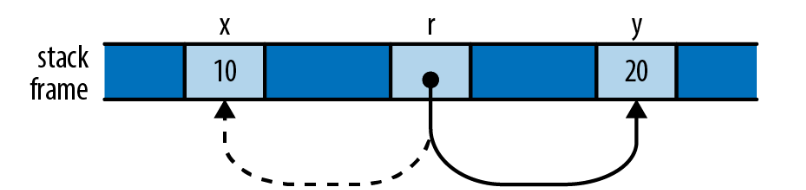
\includegraphics[width=0.8\textwidth]{../img/f5-1.png}
    \caption{引用r,现在指向y而不是x}
    \label{f5-1}
\end{figure}

代码的行为似乎太过于简单而不值一提:显然\texttt{r}现在会指向\texttt{y},因为我们把\texttt{\&y}赋给了它。但我们指出这一点是因为C++的引用与此差别很大:如之前展示的一样,在C++中对一个引用赋值会把值存储在引用指向的对象。一旦一个C++引用被初始化之后,将没有任何方法让它指向别的东西。

\subsection{引用的引用}
Rust允许引用的引用:
\begin{minted}{Rust}
    struct Point { x: i32, y: i32 }
    let point = Point { x: 1000, y: 729 };
    let r: &Point = &point;
    let rr: &&Point &r;
    let rrr: &&&Point = &rr;
\end{minted}

(我们写出引用的类型是为了看得更清楚,但你可以省略它们,Rust可以推导出这里的所有类型。)\texttt{.}运算符寻找目标时需要解引用多次:
\begin{minted}{Rust}
    assert_eq!(rrr.y, 729);
\end{minted}

在内存中,这些引用按照\hyperref[f5-2]{图5-2}的形式排布。

\begin{figure}[htbp]
    \centering
    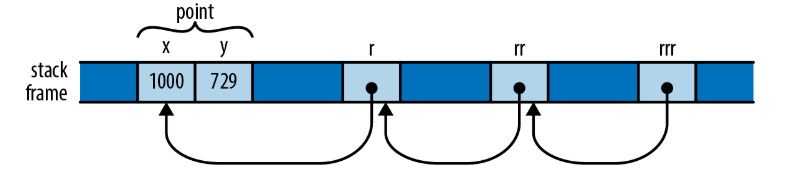
\includegraphics[width=0.8\textwidth]{../img/f5-2.png}
    \caption{引用的引用链}
    \label{f5-2}
\end{figure}

因此表达式\texttt{rrr.y},在\texttt{rrr}的类型的引导下,实际上进行了3次解引用才得到了\texttt{Point}值,然后才能获得它的\texttt{y}字段。

\subsection{比较引用}

类似于\texttt{.}运算符,Rust比较运算符“看穿”任意数量的引用嵌套:
\begin{minted}{Rust}
    let x = 10;
    let y = 10;

    let rx = &x;
    let ry = &y;

    let rrx = &rx;
    let rry = &ry;

    assert!(rrx <= rry);
    assert!(rrx == rry);
\end{minted}

这里,最后的断言会成功,尽管\texttt{rrx}和\texttt{rry}指向不同的值(\texttt{rx}和\texttt{ry}),但因为\texttt{==}运算符会解除所有的引用然后对最终的值\texttt{x}和\texttt{y}进行比较。这几乎总是你想要行为,尤其是编写泛型函数时。如果你实际上是想知道两个引用是否指向相同的内存位置,你可以使用\texttt{std::ptr::eq},它会按照地址比较引用:
\begin{minted}{Rust}
    assert!(rx == ry);              // 它们指向的对象相等
    assert!(!std::ptr:eq(rx, ry));  // 但是地址不同
\end{minted}

注意比较运算符的操作数的类型必须完全相同,包括引用:
\begin{minted}{Rust}
    assert!(rx == rrx);     // error:类型不匹配:`&i32` 和 `&&i32`
    assert!(rx == *rrx);    // Ok
\end{minted}

\subsection{引用永不为空}
Rust的引用永远不可能为空,没有类似C的\texttt{NULL}或C++的\texttt{nullptr}的值。引用没有默认初始值(不管什么类型,你不能在一个变量初始化之前使用它)并且Rust不允许把整数转换为引用(除了\texttt{unsafe}代码),因此你不能把0转换为引用。

C和C++经常使用空指针来表示没有值:例如,\texttt{malloc}函数会返回一个指向新内存块的指针,但如果没有足够的内存能够满足要求就会返回一个\texttt{nullptr}。在Rust里,如果你需要一个可能是引用可能是无的值,你可以使用类型\texttt{Option<\&T>}。在机器层面,Rust将\texttt{None}表示为空指针,将\texttt{Some(r)}(其中\texttt{r}是一个\texttt{\&T}类型的值)表示为非0的地址,因此\texttt{Option<\&T>}和C或C++中的可以为空的指针一样高效,然而它却是安全的:它的类型要求你在使用它之前要先检查它是不是\texttt{None}。

\subsection{借用任意表达式的引用}
C和C++只允许你对特定种类的表达式使用\texttt{\&}运算符,而Rust允许你借用任何表达式的引用:
\begin{minted}{Rust}
    fn factorial(n: usize) -> usize {
        (1..n+1).product()
    }
    let r = &factorial(6);
    // 算术运算符可以看穿一层引用
    assert_eq!(r + &1009, 1729);
\end{minted}

在类似这样的场景中,Rust简单的创建一个匿名变量来存储表达式的值,然后让引用指向它。匿名变量的生命周期依赖于你使用引用的方式:
\begin{itemize}
    \item 如果你立刻通过一个\texttt{let}语句把它赋值给了一个变量(或者将它变为了结构体或数组的一部分),那么Rust会让匿名变量的生命周期变得和\texttt{let}初始化的变量一样长。在上面的例子中,Rust将会对\texttt{r}引用的值进行这样的操作。
    \item 否则,匿名变量将只能生存到语句结束。在我们的示例中,存储\texttt{1009}的匿名变量只生存到\texttt{assert\_eq!}语句的结尾处。
\end{itemize}

如果你习惯于C或C++,这可能听起来很容易出错。但记住Rust永远不会让你写出产生悬垂引用的代码。如果引用被用在匿名变量的生命周期之外,Rust总是会在编译期向你报告这个问题。然后你可以把被引用的值保存在一个有恰当的生命周期的命名变量中来修复代码。

\subsection{切片和trait对象的引用}
我们至今展示的所有引用都只是简单的地址。然而,Rust还包括两种类型的\emph{胖指针}:包含值的地址和使用值所必需的额外信息的两个字的值。

切片的引用是一种胖指针,包括切片的起始地址和它的长度。我们在\hyperref[ch03]{第3章}中详细讨论了切片。

Rust的另一种胖指针类型是\emph{trait对象},一个实现了特定trait的值的引用。一个trait对象包含值的地址和一个指向该值对trait的实现的指针,用于调用trait的方法。我们将在“\hyperref[traitobject]{trait对象}”一节中详细介绍trait对象。

除了携带了这些额外信息之外,切片和trait对象的引用和我们在这一章中目前见到的所有引用一样:它们并不获取所有权,不允许比引用对象生存得更久,可能是共享或者可变的,等等。
























